\chapter{Przykładowe aplikacje}
\label{cha:przyklady}

W niniejszym rozdziale pracy zaprezentowano przykładowe aplikacje zaimplementowane w języku Erlang i uruchomione na maszynie wirtualnej opisywanej w pracy. Platformą, na której uruchamiane były przykłady był mikrokontroler LPC1769 z procesorem ARM Cortex-M3 pod kontrolą mikrojądra FreeRTOS.

Wszystkie aplikacje zostały skompilowane przy użyciu narzędzia opisanego w dodatku \ref{cha:builder}. Kody źródłowe aplikacji zostały umieszczone na płycie CD dołączonej do pracy.

\section{Silnia}
\label{sec:przykladySilnia}

\subsection{Cel aplikacji}

Aplikacja miała na celu uruchomienie przykładowego sekwencyjnego programu zaimplementowanego w języku Erlang w dwóch wersjach: z rekurencją ogonową oraz bez tego typu rekurencji.

Rekurencja ogonowa charakteryzuje się tym, że wynik wywołania funkcji rekurencyjnej całkowicie zależy od wyniku rekurencyjnego wywołania funkcji.
Nie ma zatem konieczności powrotu do poprzedniego wywołania funkcji w celu ustalenia aktualnej wartości funkcji, a co za tym idzie zapisywania na stosie adresu powrotu i wyrażeń potrzebnych do wyliczenia zwracanego wyniku.
Kompilator Erlanga automatycznie wykrywa funkcje ogonowo-rekurencyjne i optymalizuje kod pośredni pod kątem użytego rozmiaru stosu (por. np. opis instrukcji \texttt{call} i \texttt{call\_only} na liście instrukcji kodu pośredniego na str. \pageref{sec:opsOps}).

Listingi \ref{lis:fac_facERL} oraz \ref{lis:fac_fac2ERL} przedstawiają kody źródłowe dwóch funkcjonalnie równoważnych sobie funkcji (\texttt{fac/1}) obliczających silnię liczby naturalnej.

\begin{figure}
\begin{multicols}{2}
\begin{lstlisting}[style=erlang, caption=Kod modułu \texttt{fac.erl}, label=lis:fac_facERL]
-module(fac).

-export([fac/1]).

fac(0) ->
    1;
fac(N) ->
    N*fac(N-1).



\end{lstlisting}

\columnbreak

\begin{lstlisting}[style=erlang, caption=Kod modułu \texttt{fac2.erl}, label=lis:fac_fac2ERL]
-module(fac2).

-export([fac/1]).

fac(N) ->
    fac(N, 1).

fac(0, Acc) ->
    Acc;
fac(N, Acc) ->
    fac(N-1, N*Acc).
\end{lstlisting}
\end{multicols}
\end{figure}

Funkcja z modułu \texttt{fac} wykorzystuje do tego celu tradycyjną rekurencję, uzależniając wynik zwrócony przez funkcję nie tylko od rekurencyjnego wywołania samej siebie, ale także od argumentu z jakim została wywołana. 

Funkcja zaimplementowana w module \texttt{fac2} wykorzystuje dodatkowy argument, tzw. akumulator, którego aktualna wartość przekazywana jest wraz z każdym kolejnym wywołaniem, a na samym końcu zwracana.
Dzięki zastosowaniu tego podejścia funkcja ta jest ogonowo-rekurencyjna, co pozwala na optymalizację użycia stosu przez kompilator Erlanga w kodzie pośrednim.

Celem eksperymentu było uruchomienie dwóch ww. funkcji obliczających silnię dla różnych wejściowych liczb naturalnych od 1 do 200. Pozwoliło to na sprawdzenie działania podstawowych elementów maszyny wirtualnej, m.in. interpretera kodu pośredniego, \emph{garbage collectora} czy arytmetyki dużych liczb (do zapisania wyniku $200!$ potrzebnych jest 156 bajtów).


\subsection{Uzyskane wyniki}

Silnia została obliczona dla wejściowych liczb: 1, 11 (wynik $11!$ jest ostatnim, jaki mieści się na 28 bitach i może zostać przechowany jako wyrażenie typu \textbf{SMALL}), 12 (wynik $12!$ jest ostatnim, jaki mieści się na 32 bitach i jest zarazem pierwszym, który do przechowania potrzebuje typu danych \textbf{BIGNUM}), 25, 50, 75, 100, 125, 150, 175 i 200. Dla wszystkich wartości wejściowych, dla obu modułów, uzyskano poprawne wartości silni.

Obliczenia zostały wykonane w kontekście procesu Erlanga, który był jedynym uruchomionym w~tym momencie na maszynie wirtualnej.

Czas wykonania mierzony był przy użyciu sprzętowego licznika wbudowanego w mikrokontroler, taktowanego zegarem o częstotliwości 1 MHz.

Rezultaty uzyskane w trakcie uruchomień zostały zaprezentowane na rysunku \ref{fig:facGraphs}.


Zgodnie z oczekiwaniami rozmiar sterty procesu w przypadku modułu \texttt{fac} rósł znacznie szybciej niż w przypadku modułu \texttt{fac2}, osiągając aż 610 słów maszynowych
w porównaniu do 90 słów w~przypadku funkcji ogonowo-rekurencyjnej dla obliczenia wyniku $200!$.
Na samo przechowanie stosu wywołań w pierwszym przypadku konieczne jest 400 słów maszynowych (200 liczb \textbf{SMALL} i 200 adresów powrotu).

Dużo większy rozmiar sterty dla pierwszego z modułów miał bezpośredni wpływ na dużo rzadsze uruchomienia \emph{garbage collectora}.
Ponieważ wyrażenia zajmujące znaczną część sterty (duże liczby) potrzebne były tylko w czasie jednego rekurencyjnego wywołania funkcji, przy każdym jego uruchomieniu zwalniana byłą dużą część pamięci. Większa część zaalokowanej sterty mogła zostać zatem później wykorzystana przez kolejne wywołania funkcji.

Z tego samego powodu w przypadku funkcji ogonowo-rekurencyjnej, \emph{garbage collectorowi} udało zwolnić się większą część pamięci (ok. 4500 słów maszynowych w porównaniu do ok. 3500 słów maszynowych).

Sam czas wykonywania kodu był nieco większy w przypadku modułu \texttt{fac} (2981 \textmugreek s w porównaniu do 2108 \textmugreek s), co wynika bezpośrednio z większej liczby instrukcji w kodzie pośrednim.
Czas spędzony na odśmiecaniu sterty procesu (ok. 43\% łącznego czasu wykonania programu w przypadku modułu \texttt{fac2} w porównaniu do ok. 21\% czasu dla drugiego modułu) miał jednak decydujący wpływ na łączny czas obliczenia silni, który okazał się wyraźnie większy dla modułu z funkcją ogonowo-rekurencyjną (4920 \textmugreek s w porównaniu do 3750 \textmugreek s).

Dla porównania, obie powyższe funkcje obliczające silnię z 200 na maszynie wirtualnej BEAM na komputerze z systemem operacyjnym MacOS X i procesorem Intel Core i7, wykonały się w ok. 1800 \textmugreek s.
Należy wspomnieć, że początkowy rozmiar sterty procesu został ustawiony na 12 słów maszynowych, tak jak jest to w przypadku maszyny implementowanej w pracy.


Różnicę można również zauważyć w liczbie wykonanych redukcji przez procesy, która jest nieco większa w przypadku wykonywania kodu z modułu \texttt{fac}.
Powodem tego jest fakt, że w całkowitą liczbę redukcji procesu wliczany jest czas uruchomienia \emph{garbage collectora}, ale tylko w przypadku gdy jest on uruchamiany przez instrukcje z rodziny \texttt{allocate} (opkody 12-15). Jeżeli \emph{garbage collector} uruchomiony zostanie w trakcie operacji arytmetycznej, redukcje nie są doliczane.
Ponieważ kod modułu \texttt{fac2} nie używa stosu, liczba redukcji przez niego wykonana pochodzi tylko i wyłącznie z wywołań funkcji.

\begin{figure}

\begin{multicols}{2}

\begin{gnuplot}[terminal=epslatex,terminaloptions=color,scale=0.7]
	set grid
	set title 'Pamięć zwolniona przez \emph{garbage collector}'
	set ylabel 'słowa maszynowe'
	set xlabel '$n$'
	set yr [0:5000]
	set size ratio 0.8
	plot 'facstats.csv' using 1:2 w p pt 7 ps 1 title 'fac:fac($n$)',\
			'facstats.csv' using 1:2 smooth csplines lt 3 lw 4 lc 1 notitle,\
			'fac2stats.csv' using 1:2 w p pt 7 ps 1 lc 3 title 'fac2:fac($n$)', \
			'fac2stats.csv' using 1:2 smooth csplines lt 3 lw 4 lc 3 notitle
\end{gnuplot}

\begin{gnuplot}[terminal=epslatex,terminaloptions=color,scale=0.7]
	set grid
	set title 'Uruchomienia \emph{garbage collectora}'
	set ylabel 'uruchomienia'
	set xlabel '$n$'
	set yr [0:180]
	set size ratio 0.8
	plot 'facstats.csv' using 1:3 w p pt 7 ps 1 title 'fac:fac($n$)',\
			'facstats.csv' using 1:3 smooth csplines lt 3 lw 4 lc 1 notitle,\
			'fac2stats.csv' using 1:3 w p pt 7 ps 1 lc 3 title 'fac:fac2($n$)', \
			'fac2stats.csv' using 1:3 smooth csplines lt 3 lw 4 lc 3 notitle
\end{gnuplot}

\begin{gnuplot}[terminal=epslatex,terminaloptions=color,scale=0.7]
	set grid
	set title 'Czas działania'
	set ylabel 'czas ($\mu s$)'
	set xlabel '$n$'
	set size ratio 0.8
	plot 'facstats.csv' using 1:5 w p pt 7 ps 1 title 'całkowity fac:fac($n$)',\
			'facstats.csv' using 1:5 smooth csplines lt 3 lw 4 lc 1 notitle,\
			'fac2stats.csv' using 1:5 w p pt 7 ps 1 lc 3 title 'całkowity fac:fac2($n$)', \
			'fac2stats.csv' using 1:5 smooth csplines lt 3 lw 4 lc 3 notitle,\
\end{gnuplot}


\begin{gnuplot}[terminal=epslatex,terminaloptions=color,scale=0.7]
	set grid
	set title 'Wykonane redukcje'
	set ylabel 'redukcje'
	set xlabel '$n$'
	set size ratio 0.8
	plot 'facstats.csv' using 1:4 w p pt 7 ps 1 title 'fac:fac($n$)',\
			'facstats.csv' using 1:4 smooth csplines lt 3 lw 4 lc 1 notitle,\
			'fac2stats.csv' using 1:4 w p pt 7 ps 1 lc 3 title 'fac:fac2($n$)', \
			'fac2stats.csv' using 1:4 smooth csplines lt 3 lw 4 lc 3 notitle
\end{gnuplot}


\begin{gnuplot}[terminal=epslatex,terminaloptions=color,scale=0.7]
	set grid
	set title 'Rozmiar sterty procesu'
	set ylabel 'słowa maszynowe'
	set xlabel '$n$'
	set size ratio 0.8
	plot 'facstats.csv' using 1:9 w p pt 7 ps 1 title 'fac:fac($n$)',\
			'facstats.csv' using 1:9 w steps lt 3 lw 4 lc 1 notitle,\
			'fac2stats.csv' using 1:9 w p pt 7 ps 1 lc 3 title 'fac:fac2($n$)', \
			'fac2stats.csv' using 1:9 w steps lt 3 lw 4 lc 3 notitle,\
\end{gnuplot}

\begin{gnuplot}[terminal=epslatex,terminaloptions=color,scale=0.7]
	set grid
	set title 'Czas działania'
	set ylabel 'czas ($\mu s$)'
	set xlabel '$n$'
	set yr [0:4000]
	set size ratio 0.8
	plot 'facstats.csv' using 1:7 w p pt 7 ps 1 title 'kod fac:fac($n$)',\
			'facstats.csv' using 1:7 smooth csplines lt 3 lw 4 lc 1 notitle,\
			'fac2stats.csv' using 1:7 w p pt 7 ps 1 lc 3 title 'kod fac:fac2($n$)', \
			'fac2stats.csv' using 1:7 smooth csplines lt 3 lw 4 lc 3 notitle,\
			'facstats.csv' using 1:6 w p pt 5 ps 1 lc 1 title 'GC fac:fac($n$)',\
			'facstats.csv' using 1:6 smooth csplines lt 3 lw 4 lc 1 notitle,\
			'fac2stats.csv' using 1:6 w p pt 5 ps 1 lc 3 title 'GC fac:fac2($n$)', \
			'fac2stats.csv' using 1:6 smooth csplines lt 3 lw 4 lc 3 notitle
\end{gnuplot}

\end{multicols}

\caption{Porównanie wyników uruchomienia modułów \texttt{fac} oraz \texttt{fac2} na implementowanej maszynie wirtualnej.}
\label{fig:facGraphs}

\end{figure}

\subsection{Wnioski}

Eksperymentalne uruchomienia funkcji obliczających silnię zwróciły poprawne wyniki, testując w~ten sposób arymetykę dużych liczb zaimplementowaną w maszynie wirtualnej.
Zmierzone czasy wykonania zarówno kodu jak i odśmiecania mogą stanowić punkt odniesienia przy przewidywania narzutu, jaki do aplikacji uruchamianej na mikrokontrolerze może wprowadzić maszyna wirtualna.
Na ich podstawie można wyciągnąć wniosek, że rekurencja ogonowa co prawda wykorzystuje zdecydowanie mniej pamięci, jednak przez dużą liczbę odśmieceń zajmuje więcej czasu. 

W momencie projektowania funkcji w Erlangu, która uruchamiana będzie na szybkim procesorze i~przy dostępnej dużej ilości pamięci, wybór pomiędzy rekurencją ogonową a tradycyjną nie ma większego znaczenia (o ile liczba wywołań nie jest bardzo duża, mogąca spowodować skończenie się dostępnej pamięci) i wybór implementacji powinien zostać podyktowany czytelnością kodu funkcji. Jednak w przypadku urządzeń wbudowanych, ze względu na bardzo ograniczone rozmiary zasobów, zawsze powinna być wybierana rekurencja ogonowa, która po optymalizacji kompilatora nie będzie używać stosu procesu w momencie rekurencyjnych wywołań funkcji.
Wydajność konkretnej aplikacji, poprzez zmniejszenie liczby uruchomień \emph{garbage collectora}, może zostać poprawiona przez wybór w pliku konfiguracyjnym początkowego rozmiaru sterty procesu, adekwatnego do jego logiki.


\section{Kontrola diod LED przez procesy}
\label{sec:przykladyDiody}

\subsection{Cel aplikacji}

Celem aplikacji było uruchomienie przykładowego programu korzystającego ze współbieżnych cech języka Erlang na zaimplementowanej maszynie wirtualnej.
Aplikacja miała pozwolić na sprawdzenie działania takich funkcjonalności maszyny wirtualnej jak:
przesyłania i odbierania wiadomości między procesami, propagacji zakończenia działania procesu (\emph{link}), mechanizmów zarządzania czasem (przeterminowania i wysyłania wiadomości do innych procesów z opóźnieniem) czy stabilnością działania automatycznego zarządzania pamięcią.

W tym celu zaimplementowano dwa moduły: \texttt{led\_sup} i \texttt{led\_drv}, których zadaniem była kontrola diod LED, przez funkcje wbudowane kontrolujące GPIO, w dwóch kolorach: czerwonym i~zielonym.
W systemie uruchomiony był jeden proces implementujący logikę pierwszego z modułów oraz trzy procesy --- drugiego z nich.
Każdy z procesów \texttt{led\_drv} kontrolował stan jednej zielonej diody --- zapalał lub gasił ją po otrzymaniu wiadomości z procesu \texttt{led\_sup}. Proces ten, w odstępie półsekundowym, wysyłał do losowego procesu wiadomość o zmianie stanu diody. Dodatkowo, w logice procesu ustawione zostało przeterminowanie, efektem którego było zliczanie sytuacji, gdy żadna wiadomość kontrolująca stan diody nie przyszła do skrzynki odbiorczej procesu w~odstępie półtorej sekundy.
Efektem wystąpienia takiego zdarzenia piąty raz w czasie życia procesu skutkowało jego zakończeniem z błędem.

\begin{figure}[h]
\centerline{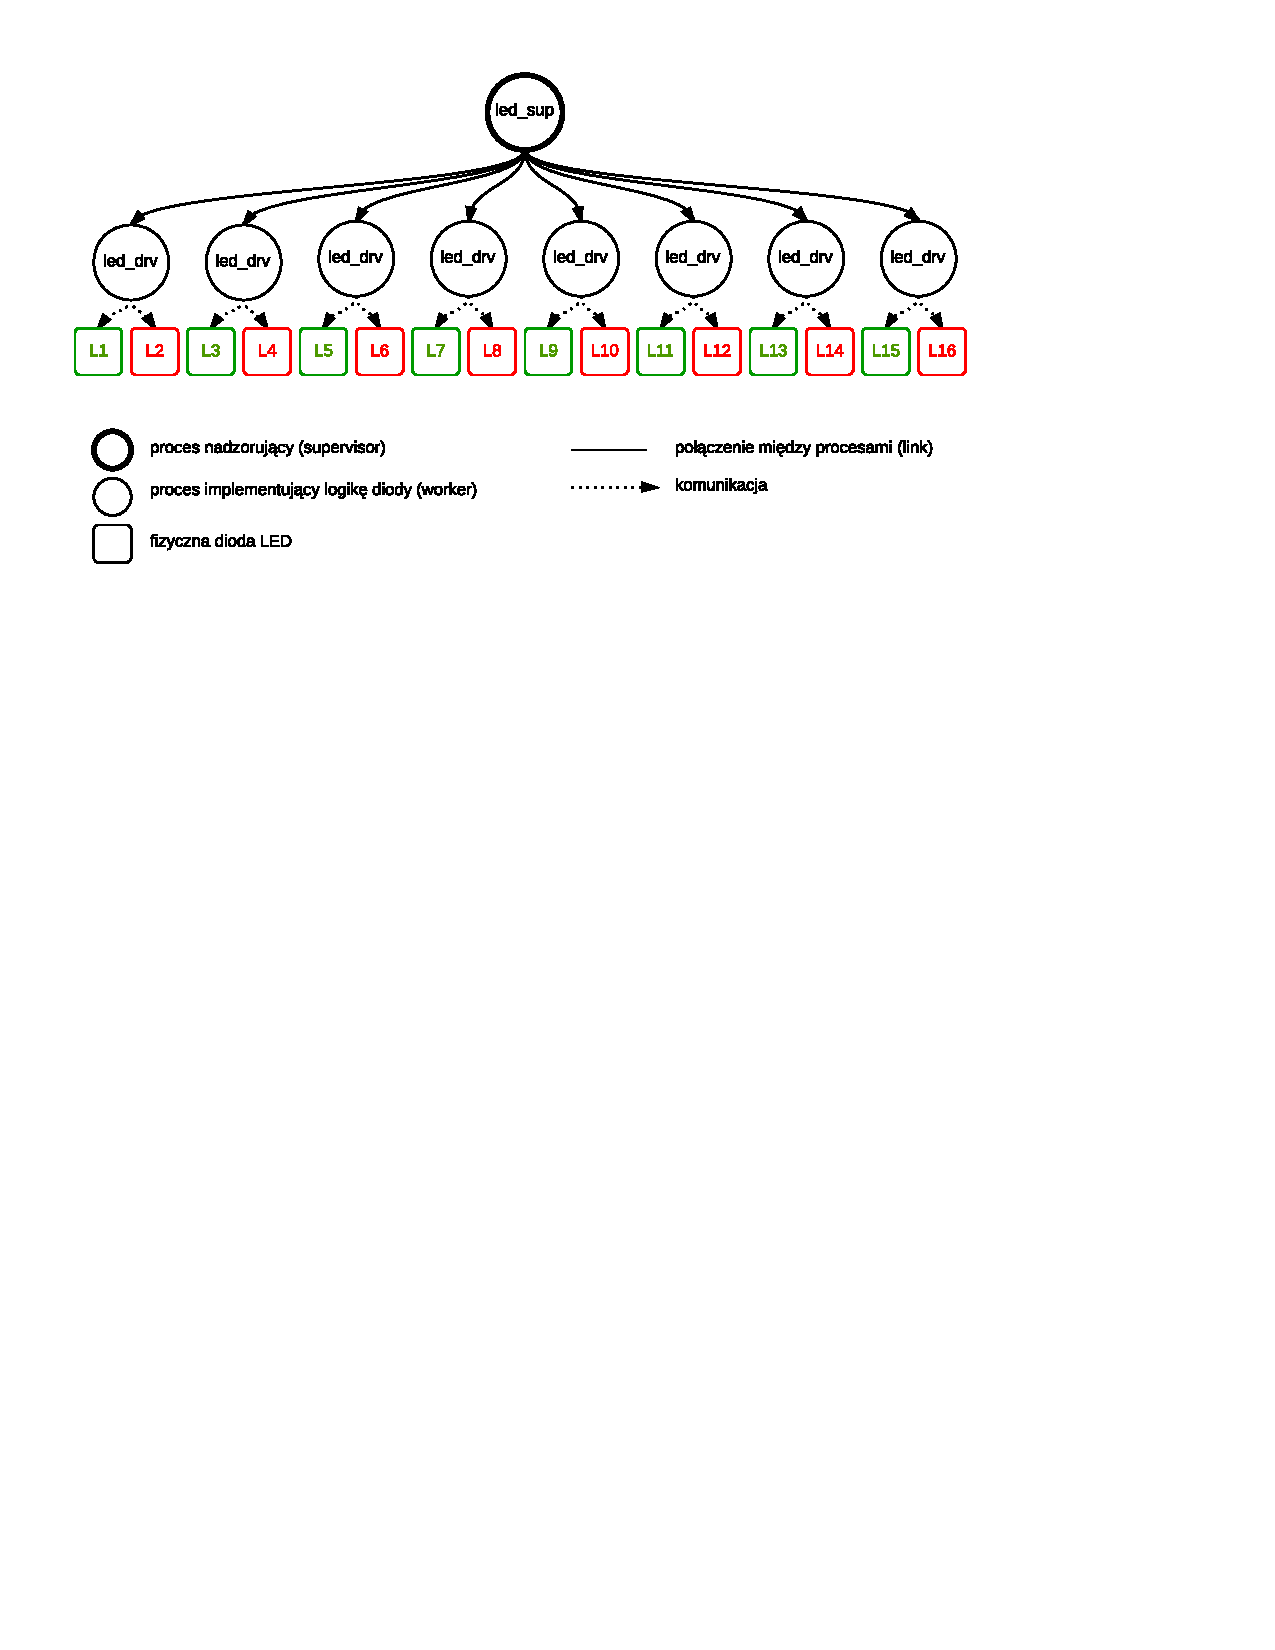
\includegraphics[scale=1, clip, trim=10mm 190mm 80mm 10mm]{example_led_processes}}
\caption{Struktura procesów w aplikacji i kontrolowanych przez nie diod}
\label{fig:exampleledprocesses}
\end{figure}

Stan systemu wizualizowały dodatkowo trzy czerwone diody, które były zgaszone w momencie gdy procesy kontrolujące odpowiadające im diody zielony były uruchomione i zapalone w przeciwnym wypadku.
Pojedynczy proces był procesem nadzorczym (\emph{supervisor}), którego zadaniem było ponowne uruchamianie kończących się procesów kontrolujących diody zielone. W tym celu, proces ten musiał działać jako proces przechwytujący wyjścia procesów z nim powiązanych jako wiadomości (co w języku Erlang realizowane jest poprzez ustawienie flagi procesu \texttt{trap\_exit} na \texttt{true}).
Dla czytelniejszej prezentacji stanu systemu w przykładzie, proces kontrolujący diodę zieloną restartowany był dopiero po upływie przynajmniej sekundy po otrzymaniu wiadomości o zakończeniu się jego poprzednika.

Kontrola przebiegu działania programu odbywała się zatem za pomocą trzech typów wiadomości przesyłanych między uruchomionymi procesami:
\begin{itemize}
\item \texttt{toggle} --- wysyłanej co pół sekundy przez proces nadzorczy do samego siebie, w efekcie czego wysyłał on taką samą wiadomość do jednego z procesów kontrolujących diody;
\item \texttt{\{restart,Id}\} --- wysyłana przez proces nadzorczy do samego siebie, z sekundowym opóźnieniem, na której skutek odebrania restartowany był odpowiedni proces kontrolujący diodę;
\item \texttt{\{'EXIT',Pid,timeout\}} --- wiadomość otrzymywana przez proces nadzorczy na skutek zakończenia działania procesu kontrolującego diodę na skutek osiągnięcia piątego przeterminowania.
\end{itemize}

Zależności między procesami uruchomionymi w ramach przykładowej aplikacji zostały zaprezentowane na rysunku \ref{fig:exampleledprocesses}. Fizyczna realizacja podłączeń diod, sterowanych stanem niskim, do mikrokontrolera wykorzystanego w przykładzie przedstawiona została na rysunku \ref{fig:exampleled}. Na obu rysunkach diody zostały oznaczone tymi samymi symbolami.



\begin{figure}[h]
\centerline{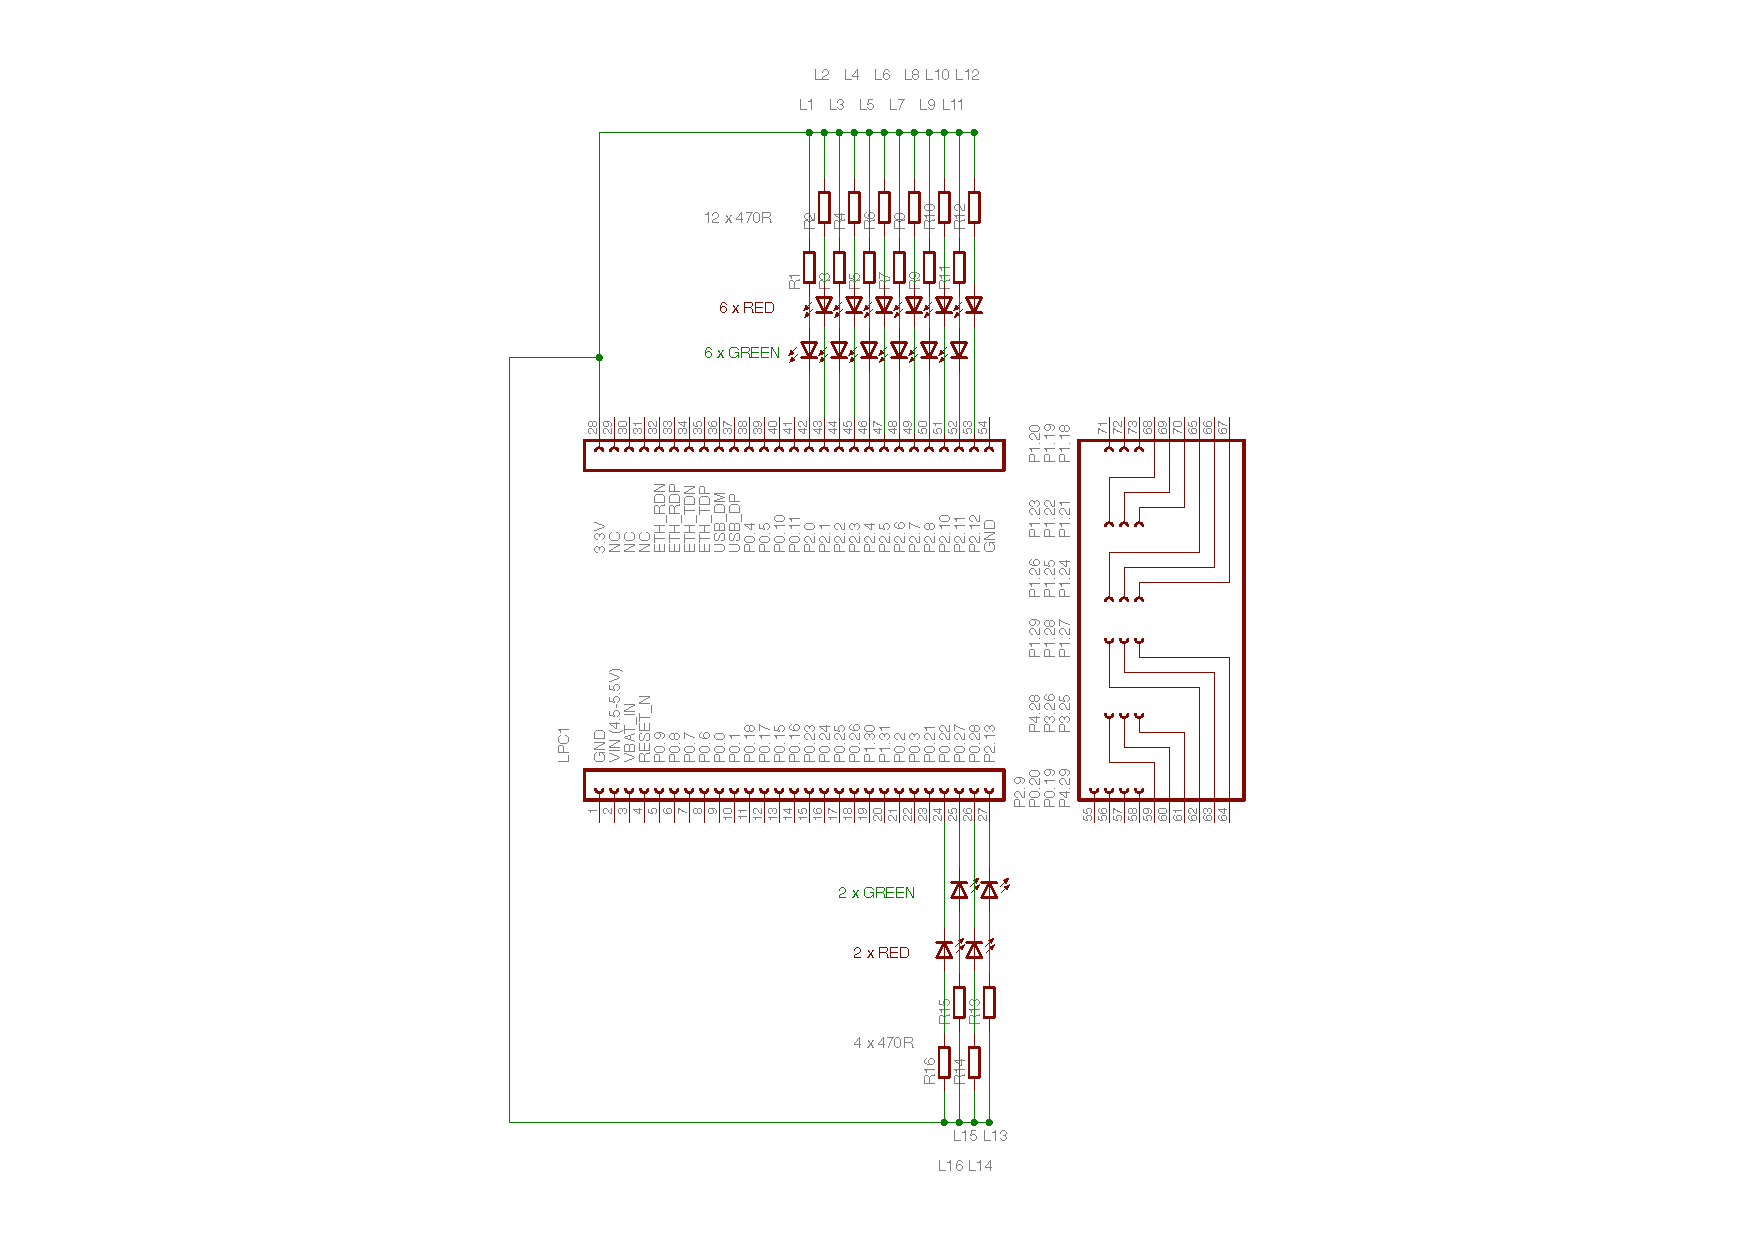
\includegraphics[scale=1, clip, trim=0mm 40mm 0mm 35mm]{example_led}}
\caption{Schemat podłączenia diod LED do płytki prototypowej z mikrokontrolerem LPC1769}
\label{fig:exampleled}
\end{figure}


\subsection{Uzyskane wyniki}

Kod aplikacji, poza wspomnianymi modułami, składał się z częściowo zaimplementowanych modułów \texttt{lists} oraz \texttt{random} zawierających funkcje pomocnicze w realizacji implementacji.
Należały do nich takie funkcje jak np. \texttt{lists:keyfind/3} czy \texttt{lists:delete/2}.

Tabela \ref{table:ledMemory} prezentuje poziom zajętości pamięci dostępnej w mikrokontrolerze przez poszczególne elementy uruchomionej maszyny wirtualnej oraz załadowanych pięciu modułów składających się na całą aplikację.

\begin{figure}[h]
\begin{longtable}{|l|l|}
\hline

\textbf{Element systemu} & \textbf{Zajęta pamięć [B]} \\
\endfirsthead
\hline
Tablica atomów (maks. 100 pozycji) & 3784 \\
\hline
Tablica eksportów (maks. 100 pozycji) & 440 \\
\hline
Funkcje wbudowane & 1040 \\
\hline
Moduły, w tym: & 11000 \\
{\small \texttt{led\_drv}} & {\small 2160} \\
{\small \texttt{led\_sup}} & {\small 5944} \\
{\small \texttt{lists}} & {\small 1656} \\
{\small \texttt{main}} & {\small 560} \\
{\small \texttt{random}} & {\small 680} \\
\hline
Pula procesów (4 procesy) & 6584 \\
\hline
\textbf{Suma} & \textbf{22848} \\
\hline

\caption{Pamięć zajęta przez poszczególne uruchomione elementy maszyny wirtualnej} 
\label{table:ledMemory} \\
\end{longtable}
\end{figure}

W trakcie testowych uruchomień systemu problemem okazało się dynamiczne tworzenie i usuwanie zadań systemu FreeRTOS.
Każda operacja tego typu wymagała alokacji nowego stosu dla zadania, który, jak udało się ustalić doświadczalnie, do prawidłowego działania powinien składać się z przynajmniej 350 słów maszynowych.
Częste zwalnianie pamięci procesów, które kończą swoje działanie i alokacja pamięci dla nowotworzonych procesów prowadziły do fragmentacji pamięci. W efekcie, np. pomimo dostępnych ponad 5 kB pamięci RAM nie można było zaalokować obszaru pamięci dla stosu przeznaczonego dla nowego procesu.
Rozwiązaniem tego problemu okazało się utworzenie, zaalokowanej na samym początku działania maszyny wirtualnej, puli zadań systemu FreeRTOS do których przypisywane były procesy tworzone w trakcie działania systemu.
Wobec powyższego, w trakcie uruchomienia aplikacji jedynymi dynamicznie zarządzanymi obszarami pamięci były sterty procesów i wiadomości przesyłane między procesami, będące na tyle niewielkie w stosunku do dostępnej pamięci, że nie powodowały fragmentacji pamięci.

W celu sprawdzenia stabilności działania maszyny wirtualnej pod kątem realizacji przeterminowań a~także ewentualnych wycieków pamięci powodowanych przez \emph{garbage collector} przykładową aplikację pozostawiono uruchomioną na 12 godzin.
Następnie zestawiono zbiór statystyk zbieranych przez uruchomioną maszynę wirtualną co minutę w czasie jej uruchomienia.
Statystyki te zaprezentowano w~formie wykresów na rysunku \ref{fig:ledGraphs}.

\begin{figure}
\begin{gnuplot}[terminal=epslatex,terminaloptions=color]
	set grid
	set title 'Liczba uruchomionych procesów'
	set ylabel 'procesy'
	set xlabel '$t$ [min]'
	set yr [0:5]
	set xr [0:720]
	set size 1.3,0.6
	plot 'led_12h.csv' using 11:2 w p pt 7 ps 1 notitle
\end{gnuplot}

\begin{gnuplot}[terminal=epslatex,terminaloptions=color]
	set grid
	set title 'Dostępna pamięć RAM'
	set ylabel 'dostępna pamięć [B]'
	set xlabel '$t$ [min]'
	set yr [0:4000]
	set xr [0:720]
	set size 1.3,0.6
	plot 'led_12h.csv' using 11:3 w p pt 7 ps 1 notitle
\end{gnuplot}

\begin{gnuplot}[terminal=epslatex,terminaloptions=color]
	set grid
	set title 'Łączny rozmiar sterty procesów'
	set ylabel 'rozmiar sterty [słowa maszynowe]'
	set xlabel '$t$ [min]'
	set yr [0:150]
	set xr [0:720]
	set size 1.3,0.6
	plot 'led_12h.csv' using 11:4 w p pt 7 ps 1 notitle
\end{gnuplot}

\begin{gnuplot}[terminal=epslatex,terminaloptions=color]
	set grid
	set title 'Liczba uruchomień \emph{garbage collectora}'
	set ylabel 'uruchomienia'
	set xlabel '$t$ [min]'
	set xr [0:720]
	set size 1.3,0.6
	plot 'led_12h.csv' using 11:6 w p pt 7 ps 1 notitle
\end{gnuplot}
\end{figure}

\begin{figure}
\begin{gnuplot}[terminal=epslatex,terminaloptions=color]
	set grid
	set title 'Pamięć zwolniona przez \emph{garbage collector}'
	set ylabel 'zwolniona pamięć [słowa maszynowe]'
	set xlabel '$t$ [min]'
	set xr [0:720]
	set size 1.3,0.6
	plot 'led_12h.csv' using 11:5 w p pt 7 ps 1 notitle
\end{gnuplot}

\begin{gnuplot}[terminal=epslatex,terminaloptions=color]
	set grid
	set title 'Liczba wysłanych wiadomości'
	set ylabel 'wiadomości'
	set xlabel '$t$ [min]'
	set xr [0:720]
	set size 1.3,0.6
	plot 'led_12h.csv' using 11:8 w p pt 7 ps 1 notitle
\end{gnuplot}

\begin{gnuplot}[terminal=epslatex,terminaloptions=color]
	set grid
	set title 'Liczba wystartowanych procesów'
	set ylabel 'procesy'
	set xlabel '$t$ [min]'
	set xr [0:720]
	set size 1.3,0.6
	plot 'led_12h.csv' using 11:10 w p pt 7 ps 1 notitle
\end{gnuplot}

\caption{Wyniki uruchomienia aplikacji kontrolującej stan diod LED za pomocą dedykowanych procesów.}
\label{fig:ledGraphs}

\end{figure}

Różna liczba uruchomionych procesów w czasie zależna jest od liczby procesów oczekujących na ponowne uruchomienie w momencie dokonania odczytu statystyki.
Co za tym idzie, wahania widoczne są również na wykresie przedstawiającym rozmiar pamięci zajmowanej przez sterty wszystkich uruchomionych procesów oraz rozmiar wolnej pamięci RAM w systemie.
Niemniej, wskazania wszystkich wymienionych w czasie znajdowały się w tym samym zakresie przez cały czas działania aplikacji.
Z kolei takie wartości jak: liczba uruchomień \emph{garbage collectora}, rozmiar pamięci odzyskanej przez niego, sumaryczna liczba wysłanych wiadomości przez procesy czy sumaryczna liczba wystartowanych procesów w systemie przez cały czas działania aplikacji rosły liniowo.
Świadczy to o stabilnej i~poprawnej obsłudze aplikacji przez maszynę wirtualną wraz z upływem czasu.

\subsection{Wnioski}

Szczególną uwagę należy zwrócić na rozmiar pamięci zajmowanej przez takie elementy maszyny wirtualnej jak tablica atomów czy załadowany kod modułów.
Tablica atomów, łącznie z ok. 50 atomami załadowanymi do pamięci po starcie maszyny wirtualnej, które potrzebne są do umieszczenia funkcji wbudowanych w tablicy eksportowanych funkcji, zajmuje prawie 4 kB pamięci RAM.  
Kod modułów, a w szczególności modułu \texttt{led\_sup} zajął w pamięci prawie 6 kB pomimo niezbyt skomplikowanej logiki. Wprowadza on jednak do systemu pewne złożone wyrażenia (jak lista diod) oraz znaczącą liczbę nowych atomów.

Do wystartowania całej maszyny wirtualnej z przykładową aplikacją potrzebne było ponad 22 kB pamięci z dostępnych 28 kB.
Należy więc wysunąć wniosek, że tak ograniczony rozmiar pamięci RAM, jak w przypadku mikrokontrolera LPC1769, będzie przeszkodą w implementacji kolejnych funkcji wbudowanych oraz programów o bardziej skomplikowanej logice, a co za tym idzie dłuższym kodzie pośrednim i z większą ilością uruchomionych procesów aniżeli w przypadku opisanych w niniejszym rozdziale przykładowych aplikacji.

Z kolei uzyskane wyniki długoterminowego testu, jakim było uruchomienie przykładowego programu przez czas dwunastu godzin świadczą o stabilnym działaniu: mechanizmów zarządzania czasem, algorytmu odśmiecania pamięci, zarządzania współbieżnym wykonywaniem logiki procesów oraz mechanizmu komunikacji pomiędzy procesami zaimplementowanych w ramach maszyny wirtualnej Erlanga dla systemu FreeRTOS.

\section{Sterownik RFM73}
\label{sec:przykladyRfm}

\subsection{Cel aplikacji}

Celem aplikacji było zaimplementowanie biblioteki sterownika do modułu radiowego RFM73 \cite{RFM73}, produkowanego przez firmę Hope Microelectronics.
Ten tani układ (koszt jednej sztuki to ok. 10 PLN) pozwala na komunikację bezprzewodową w paśmie 2,4 GHz z szybkością dochodzącą do 2 Mbps. Warstwa sprzętowa zapewnia możliwość wysłania pakietu składającego się z maksymalnie 32 bajtów.
Odpowiedzialność za implementację protokołu pozwalającego na wysyłanie dłuższych pakietów należy już jednak do programisty.

Moduł komunikuje się ze światem zewnętrznym dzięki wbudowanemu w niego mikrokontrolerowi, za pomocą interfejsu szeregowego SPI (\emph{Serial Peripheral Interface}). Sam układ zapewnia także sprawdzanie poprawności pakietu za pomocą sumy kontrolnej, prosty mechanizm retransmisji czy adresowania urządzeń w sieci.

Typowymi zastosowaniami modułu mogą być takie urządzenia jak np:
\begin{itemize}
\item urządzenia zdalnego sterowania;
\item sensory przesyłające dane pomiarowe;
\item urządzenia peryferyjne do komputerów osobistych.
\end{itemize}

Implementowana aplikacja miała pozwolić na przykładowe obsłużenie urządzenia peryferyjnego w~języku Erlang, w tym wypadku za pomocą zaimplementowanych funkcji wbudowanych obsługujących interfejs SPI.
Funkcjonalność wyprowadzeń z modułu RFM73 pozwoliły również na zaimplementowanie biblioteki w ten sposób, by możliwe było przetestowanie tłumaczenia przerwań zewnętrznych zgłaszanych do mikrokontrolera na wiadomości wysyłane do procesów.

Fizyczna realizacja podłączeń układu do płytki uruchomieniowej z mikrokontrolerem LPC1769, na którym uruchamiany był niniejszy przykład została zaprezentowana na rysunku \ref{fig:examplerfm}.

\begin{figure}[h]
\centerline{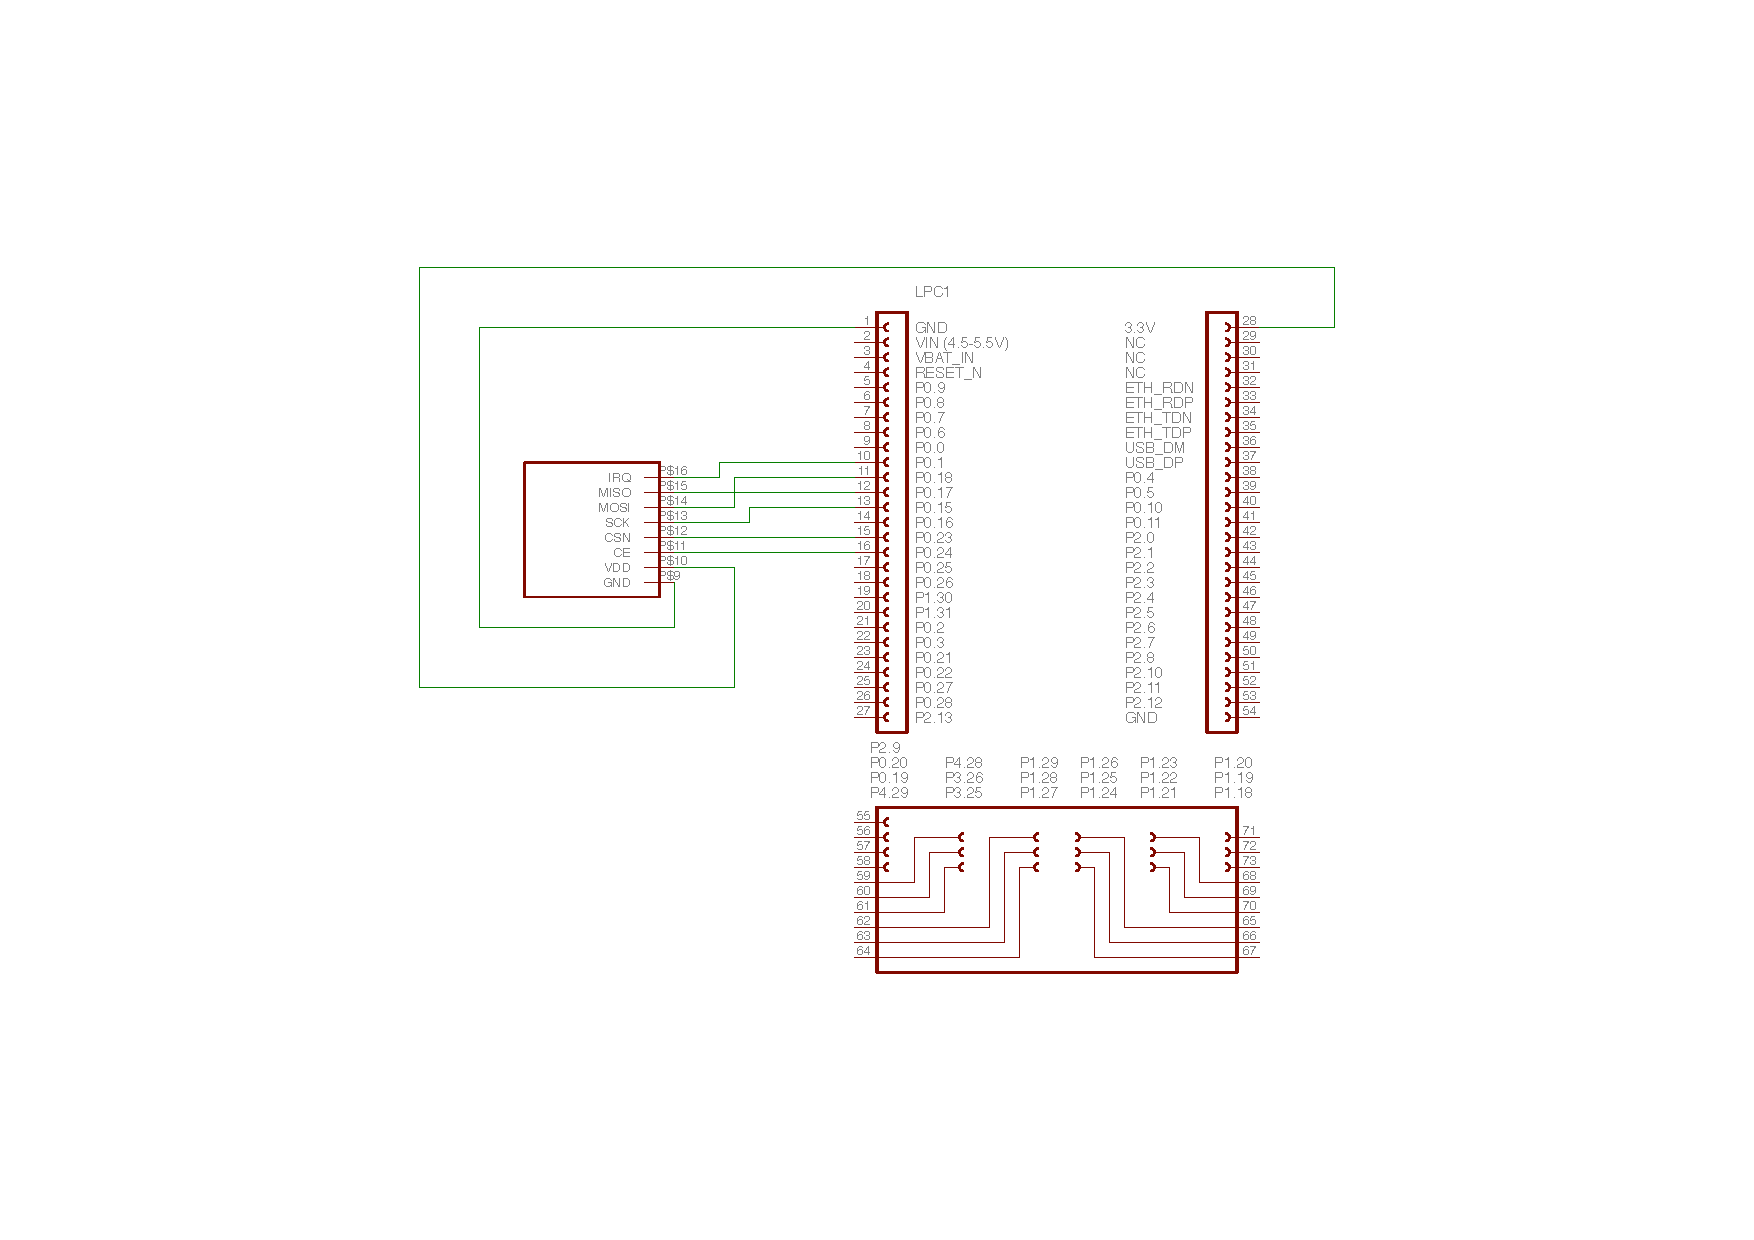
\includegraphics[scale=1, clip, trim=0 40mm 0 40mm]{example_rfm}}
\caption{Schemat podłączenia modułu RFM73 do płytki prototypowej z mikrokontrolerem LPC1769}
\label{fig:examplerfm}
\end{figure}


\subsection{Uzyskane wyniki}

Implementowany sterownik miał zapewnić abstrakcję modułu RFM73 z poziomu aplikacji napisanej w~języku Erlang z interfejsem pozwalającym na łatwe wysyłanie i odbieranie wiadomości drogą radiową.
W celu przetestowania działania modułu, wysłano zestaw krótkich pakietów do innego urządzenia z podłączonym modułem tego samego typu.
Z punktu widzenia zaimplementowanej aplikacji, pakiety te miały postać listy \texttt{"ping"}. Zostały one jednak przetworzone w taki sposób, że do bufora wiadomości modułu zapisany został ciąg bajtów odpowiadający kodom ASCII kolejnych znaków napisu.
Urządzenie odbiorze kontrolowane było przez innego rodzaju mikrokontroler --- ATmega8A, dla którego sterownik modułu RFM73 został zaimplementowany w języku C.
Program odbierający wiadomości po drugiej stronie na wiadomości o treści \texttt{"ping"} odpowiadał pakietem o treści \texttt{"pong"}.
Odebranie wiadomości przez moduł sygnalizowane było przerwaniem na wyprowadzeniu \textbf{IRQ}, podłączonym do pinu \textbf{P0.1} mikrokontrolera LPC1769.
Przerwanie było tłumaczone na wiadomość o treści \texttt{interrupt}, wysyłaną do uruchomionego procesu sterownika, co stanowiło sygnał że proces może wykonać odczyt wiadomości z kolejki modułu RFM73.
Odebrana wiadomość, przekształcona tym razem z ciągu bajtów w listę, była argumentem obiektu funkcyjnego, który został przekazany do procesu sterownika w momencie jego startu.
W niniejszym przykładzie lambda ta wypisywała w konsoli aktualny czas (wynik wywołania funkcji \texttt{erlang:now/0}) oraz listę będącą otrzymaną wiadomością.
Wynik jej działania możliwy jest do zaobserwowania na rysunku \ref{fig:consolerfm}.
Należy zauważyć, że odstęp między otrzymanymi wiadomościami jest większy niż jedna sekunda ze względu na opóźnienie, jakie wprowadziło samo wypisywanie wyjścia.

\begin{figure}[h]
\centerline{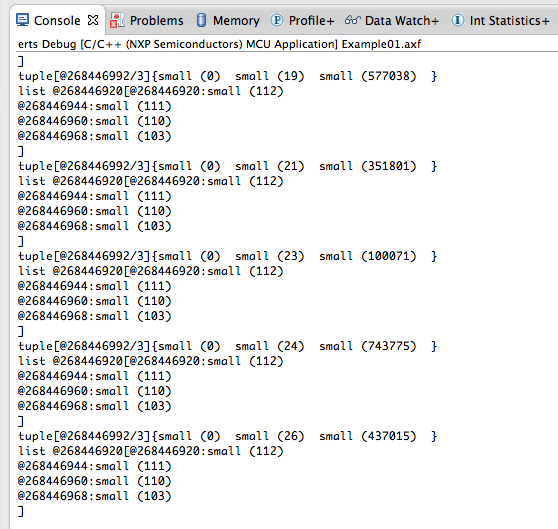
\includegraphics[scale=0.7]{console_rfm}}
\caption{Informacja w konsoli o wiadomościach postaci \texttt{"ping"} przez proces}
\label{fig:consolerfm}
\end{figure}


\subsection{Wnioski}
Aplikacja jest przykładem implementacji obsługi urządzenia peryferyjnego, z wykorzystaniem szeregowego interfejsu SPI, przez maszynę wirtualną Erlanga dla systemu FreeRTOS.
Analogicznie, obsłużone mogą zostać inne interfejsy obsługiwane przez dany mikrokontroler, jak np. UART. 

Sama implementacja sterownika z kolei może służyć do tworzenia aplikacji wykorzystujących komunikację bezprzewodową, opartą o wysokie częstotliwości, w praktyce.
Zaimplementowana biblioteka może być również podstawą do implementacji protokołu \emph{Distributed Erlang}, dzięki któremu możliwy byłby do uruchomienia klaster urządzeń komunikujących się za pomocą modułu RFM73.